\section{Verifica di ipotesi, t-statistica e p-value}

\subsection{Verifica d'ipotesi}

Lo standard error può essere utilizzata per effettuare la \textit{verifica d'ipotesi} su i coefficienti. La verifica di ipotesi più comune riguarda la verifica dell'\textit{ipotesi nulla}

\begin{equation}
H_0: \text{non c'è relazione tra X e Y}
\end{equation}

contro l'\textit{ipotesi alternativa}

\begin{equation}
H_1: \text{c'è qualche relazione tra X e Y}.
\end{equation}

Dal punto di vista matematico, questo corrisponde a testare

\begin{equation}
H_0: {\beta}_1 = 0
\end{equation}

contro

\begin{equation}
H_1: {\beta}_1 \neq 0
\end{equation}

visto che se ${\beta}_1 = 0$ allora il modello si riduce a $Y = {\beta}_0 + \epsilon$, e $X$ non è associata con Y. Per verificare l'ipotesi nulla dobbiamo determinare se $\overline{{\beta}_1}$, la nostra stima di ${\beta}_1$, è sufficientemente distante da $0$, in modo che possiamo essere sicuri che ${\beta}_1$ non sia zero. Questo dipende dall'accuratezza di ${\beta}_1$, che dipende da $SE({\beta}_1)$. Se è piccolo allora anche valori relativamente piccoli di ${\hat{\beta}}_1$ possono fornire una forte evidenza che ${\beta}_1 \neq 0$ e quindi che c'è una relazione tra $X$ e $Y$. Al contrario, se $SE({\beta}_1)$ è grande allora ${\hat{\beta}}_1$ deve essere grande in valore assoluto per poter rigettare la nostra ipotesi nulla.

\subsection{t-statistica}

In pratica, calcoliamo la \textit{t-statistica}, data da

\begin{equation}
t = \frac{{\hat{\beta}}_1 - 0}{SE({\hat{\beta}}_1)}
\end{equation}

che misura il numero di deviazioni standard di ${\hat{\beta}}_1$ che differiscono da $0$ e che sotto l'ipotesi nulla ha distribuzione $t_{n-2}$. Se non c'è alcuna relazione tra X e Y, allora ci aspettiamo che l'equazione precedente abbia una \textit{t-distribuzione} con $n - 2$ gradi di libertà. La distribuzione ha una forma a campana e per valori di $n$ più grandi di 30 è molto simile alla distribuzione normale.

Si rifiuta l'ipotesi nulla al livello di significatività $\alpha$ prefissato se il valore osservato di t

\begin{equation}
|t^{oss}| > t_{{\alpha}/2;n-2}.
\end{equation}

I test per valutare se un parametro si possa considerare pari a 0 si chiamano \textit{test di significatività}.

La verifica d'ipotesi precedente si applica anche nel caso in cui si testino valori di ${\beta}_1$ e (${\beta}_0$) diversi da 0. In generale per $H_0: {\beta}_1 = {{\beta}_1}^{H_0}$ contro ${\beta}_1 \neq {{\beta}_1}^{H_0}$ si usa la statistica test

\begin{equation}
t = \frac{{\hat{\beta}}_1 - {{\beta}_1}^{H_0}}{SE({\hat{\beta}}_1)}
\end{equation}

che sotto l'ipotesi nulla ha distribuzione $t_{n-2}$.

\subsection{p-value}

È semplice calcolare la probabilità di osservare un valore maggiore o uguale di $|t|$, assumendo ${\beta}_0$. Chiamiamo questa probabilità \textit{p-value}. Interpretiamo il p-value come segue: un valore piccolo indica che è improbabile osservare un'associazione sostanziale tra il predittore e la reazione per caso, in assenza di una reale associazione tra il predittore e la reazione. Rifiutiamo l'ipotesi nulla (dichiariamo che esiste una relazione tra $X$ e $Y$) se il p-value è sufficientemente piccolo.

\begin{figure}[H]
\centering
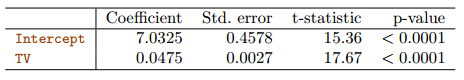
\includegraphics[scale=0.5]{t_stat_p_value}
\end{figure}